% require: pdflatex, I recommend graphics in pdf (pdfcairo driver)
\documentclass[12pt,justified,a4paper,twoside,symmetric,titlepage]{tufte-book}

\usepackage[bahasa]{babel}
\usepackage{color,graphicx,hyperref,float,algorithmic,colortbl,epigraph}
\usepackage{lipsum}

\setcounter{secnumdepth}{1}
\epigraphrule 0pt
\hypersetup{colorlinks=true,allcolors=blue}

\floatstyle{ruled}
\newfloat{algorithm}{tbp}{loa}
\providecommand{\algorithmname}{Algoritma}
\setcounter{algorithm}{0}
\renewcommand{\thealgorithm}{\arabic{algorithm}}
\floatname{algorithm}{\protect\algorithmname}

\newfloat{example}{tbp}{loa}
\providecommand{\examplename}{Contoh}
\setcounter{example}{0}
\renewcommand{\theexample}{\arabic{example}}
\floatname{example}{\protect\examplename}

\title{Judul Buku}
\author{P.~E.~Nulis}
\date{2021}

\begin{document}
\pagenumbering{roman}
\maketitle
\tableofcontents
\addcontentsline{toc}{chapter}{Daftar Isi}
\listoffigures
\addcontentsline{toc}{chapter}{Daftar Gambar}
\listoftables
\addcontentsline{toc}{chapter}{Daftar Tabel}

\chapter*{Pengantar}
\addcontentsline{toc}{chapter}{Pengantar}
\lipsum

\part{Konsep Dasar}
\pagenumbering{arabic}

\chapter{Pendahuluan}

\epigraph{\itshape Siapa yang bertemu denganku di dalam mimpi, maka sungguh dia benar-benar bertemu denganku.}{\bfseries Hadits}

\begin{marginfigure}
\label{gbrMargin}
\begin{center}
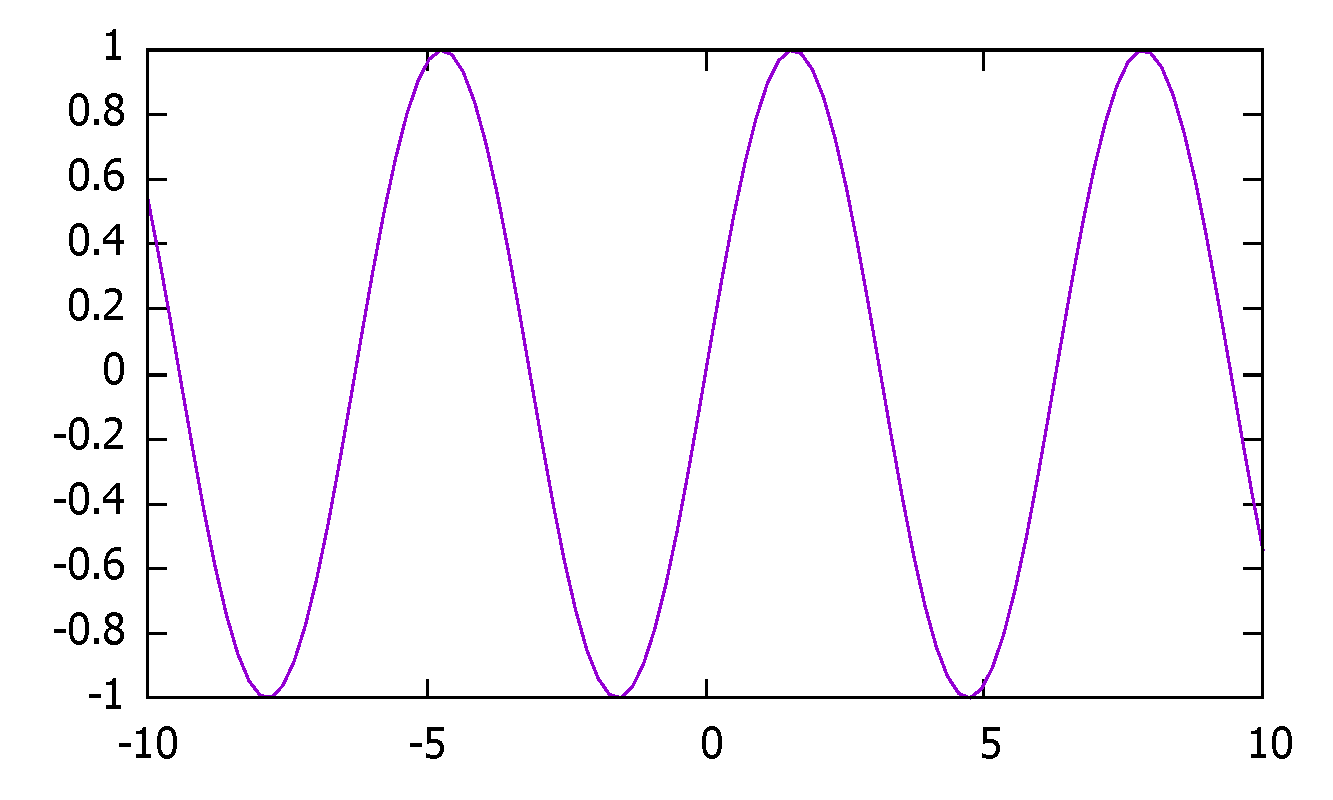
\includegraphics[width=\textwidth]{plotsinus.pdf}
\end{center}
\caption{Plot $\sin\,x$ di margin.}
\end{marginfigure}

\lipsum[1-3]\sidenote{\itshape This is a \textbf{side note}. Light curve preparation, choose an estimator, create custom bla bla bla.}

\begin{algorithm}
\caption{Algoritma kedua}
\label{algKedua}

\begin{algorithmic}[1]
\STATE Light curve preparation
\STATE Choose an estimator
\end{algorithmic}
\end{algorithm}

\lipsum[1-3]\marginnote{\itshape This is a \textbf{margin note}, not a side note. Light curve preparation, choose an estimator, create custom bla bla bla.}

\begin{algorithm}
\caption{Metode bagidua}
\label{algContoh}

\begin{algorithmic}[1]
\STATE Light curve preparation
\STATE Choose an estimator
\end{algorithmic}
\end{algorithm}

\begin{example}
\caption{Pemakaian \textit{example environment} sebagai contoh}
\label{cthContoh}

\lipsum[3]
\end{example}

\begin{figure}
\label{gbrContoh}
\begin{center}
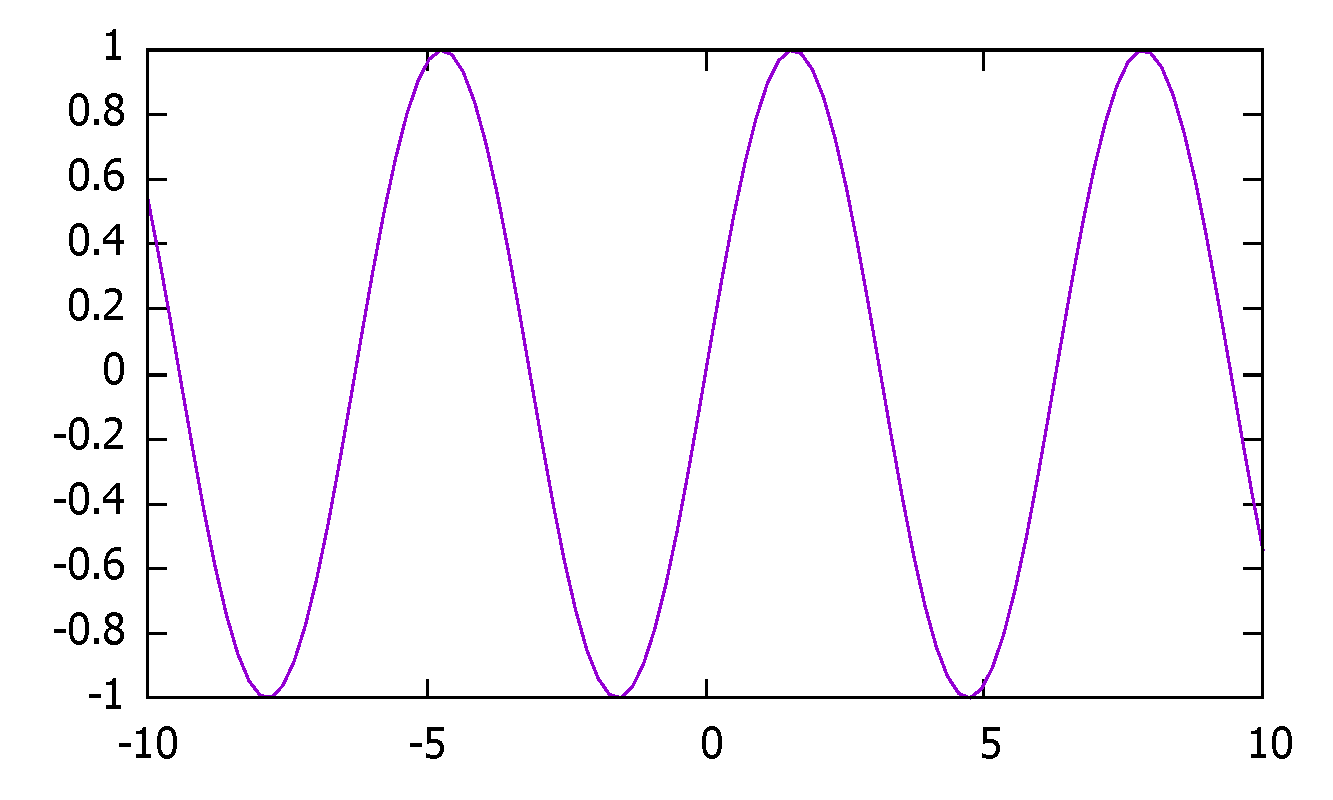
\includegraphics[width=\textwidth]{plotsinus.pdf}
\end{center}
\caption{Plot $\sin\,x$.}
\end{figure}

\lipsum[4-6]

\begin{table}
\label{tabContoh}
\caption{Tabel berwarna.}
\begin{center}
\begin{tabular}{cll}
\rowcolor{darkgray}\multicolumn{1}{c}{\textcolor{white}{No}} & \multicolumn{1}{c}{\textcolor{white}{Fungsi proxy}} & \multicolumn{1}{c}{\textcolor{white}{Centroid}}\\
\rowcolor{lightgray}1 & Manhattan & median\\
\rowcolor{gray}2 & Euclidean & mean
\end{tabular}
\end{center}
\end{table}

\lipsum[2]

See Table~(\ref{tabContoh}), or Figure~(\ref{gbrContoh}), Example~(\ref{cthContoh}), or Algorithm~(\ref{algContoh}) and  Algorithm~(\ref{algKedua}). As you can refer to model\cite{stepien2002} and an example of model repository\cite{siess2000}.

\begin{figure*}
\label{gbrPenuh}
\begin{center}
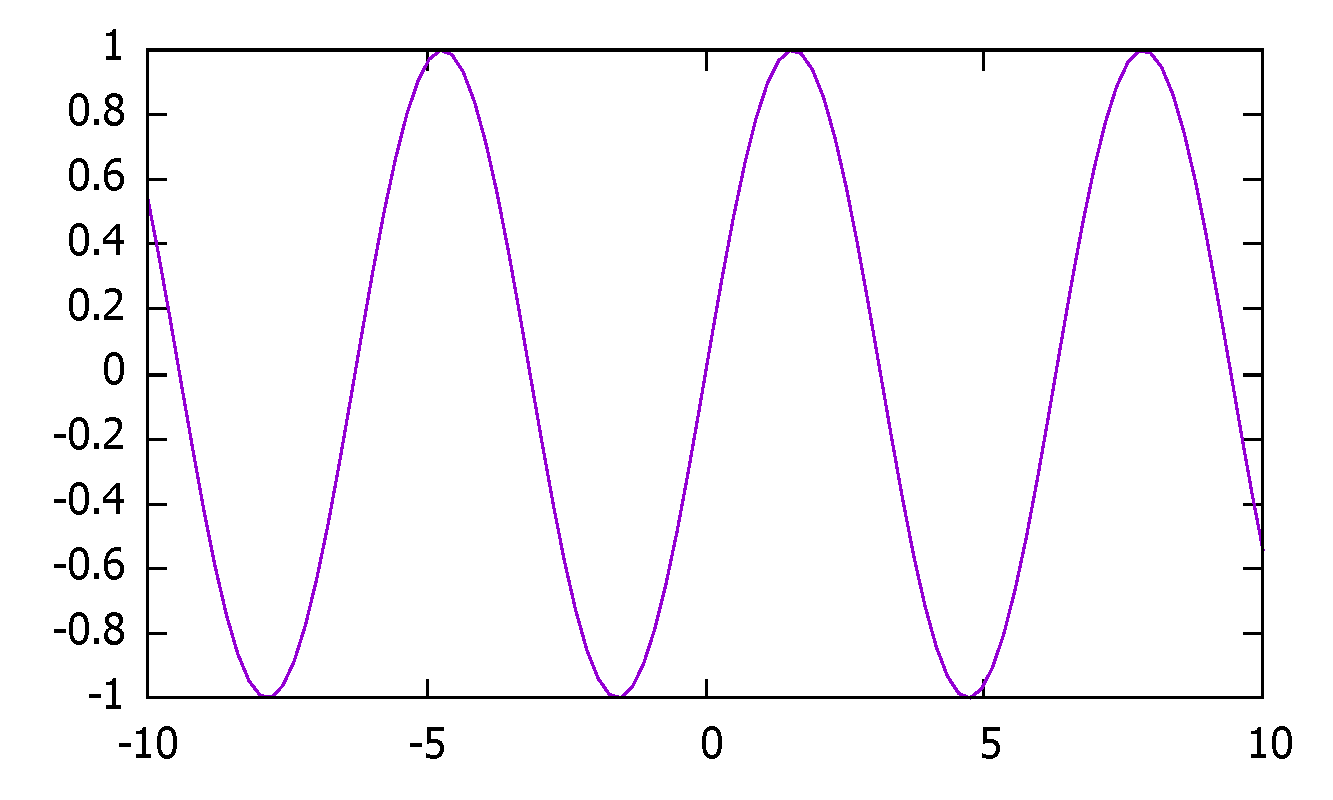
\includegraphics[width=\textwidth]{plotsinus.pdf}
\end{center}
\caption{Plot $\sin\,x$ secara penuh selebar teks.}
\end{figure*}

\lipsum[1-6]

\section{Full width text}

\begin{fullwidth}
\lipsum[1-3]
\end{fullwidth}

\lipsum[3]

\appendix

\part{Lampiran}

\chapter{Data}
\lipsum

\bibliography{bib4tufteAS}
\bibliographystyle{authordate1}

\end{document}